\documentclass[ma3408.tex]{subfiles}
\begin{document}
\chapter{Homotopy theory}
\section{Review of basics on homotopy theory}
We begin with a recollection of some facts that have been covered in Algebraic Topology I and Introduction to Topology. 
\begin{Not}
We let $I = [0,1]$ denote the unit interval. For a pointed topological space $X$ we will denote the basepoint by $x_0$ or $\ast$. 
\end{Not}
We recall the following definition. 
\begin{Def}
	A homotopy between $f,g \colon X \to Y$ is a continuous function $H \colon X \times I \to Y$ such that $H(x,0) = f(x)$ and $H(x,1) = g(x)$ and $H(x_0,t) = y_0$ for all $t \in I$. We will write $f \simeq g$, or $f \simeq_H g$, if we need to make the choice of homotopy clear. \begin{marginfigure} \centering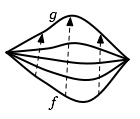
\includegraphics[scale = 0.5]{path_homotopy}\caption{A homotopy between $f$ and $g$.}\label{fig:marginfig}\end{marginfigure}

	For a subspace $A \subseteq X$, a relative homotopy is a homotopy with $H(a,t) = f(a) = g(a)$ for all $a \in A, t \in I$. 
	\end{Def}

\begin{Rem}
	Equivalently, we can specify a family of continuous maps $h_t \colon X \to Y$ such that $h_0 = f , h_1 = g$ and
\[
\begin{split}
H &\colon X \times I \to Y\\
 (x,t) &\mapsto h_t(x)
\end{split}
\]
is continuous. We will switch between the two equivalent definitions without comment, using whatever is more convenient. 
\end{Rem}
\begin{Prop}
For all spaces $X$ and $Y$, homotopy is an equivalence relation on the set of maps from $X$ to $Y$. Furthermore, if we are given $k \colon A \to X,\ell \colon Y \to B$ and homotopic maps $f \simeq g \colon X \to Y$, then $fk \simeq gk \colon A \to Y$ and $\ell f \simeq \ell g \colon X \to B$. 
\end{Prop}
\begin{proof}
Let $f,g \colon X \to Y$, then
\begin{enumerate}
	\item $f \simeq_F f$ via $F(x,t) = f(x)$ for all $x \in X,t \in I$. 
	\item If $f \simeq_F g$, then $g \simeq_G f$ where $G(x,t) = F(x,1-t)$. 
	\item If $f \simeq_F g$ and $g \simeq_G h$, then $f \simeq_H h$ via
	\[
H(x,t) = \begin{cases}
F(x,2t) & \text{ if } 0 \le t \le 1/2 \\
G(x,2t-1) & \text{ if } 1/2 \le t \le 1. 
\end{cases}
	\]
\end{enumerate}
For the last part of the proposition let $f_t$ be a homotopy between $f$ and $g$, then $f_tk$ and $\ell f_t$ give the required homotopy. 
\end{proof}
\begin{Def}
For a map $f \colon X \to Y$, we let $[f]$ denote the equivalence class containing $f$. The collection of all homotopy classes of maps from $X$ to $Y$ is denoted $[X,Y]$.\sidenote{If our spaces are based, then these should be homotopy classes of \emph{based} maps.} 
\end{Def}
\begin{Rem}
Note that if $\alpha = [f] \in [Y,Z]$ and $\beta = [g] \in [X,Y]$, then $\alpha\beta = [f \circ g] \in [X,Z]$, i.e., we can form the category $hTop_*$ whose objects are topological spaces, and whose morphisms are homotopy classes of maps. 
\end{Rem}
\begin{Rem}
We now very quickly review a number of standard topological constructions. 
\begin{itemize}
	\item Let $X$ be a space and $A \subseteq X$. A map $r \colon X \to A$ such that $r(a) = a$ for all $a \in A$ is called a retraction of $X$ onto $A$, and $A$ is called a retract of $X$. 
	\item Let $i \colon A \hookrightarrow X$ be the inclusion, so that $ri = \text{id}_A$. If $ir \simeq \text{id}_X$, we call this a deformation retraction, and say that $A$ is a deformation retract of $X$. 
	\item If $f \colon X \to Y$, then a section of $f$ is a map $s \colon Y \to X$ such that $f \circ s = \text{id}_Y$. We can also ask for a \emph{homotopy} section by requiring only that $f \circ s \simeq \text{id}_Y$. 
\end{itemize}
\end{Rem}
\begin{Def}
A map $f \colon X \to Y$ is called null-homotopic if $f \colon c_y \colon X \to Y$ where $c_y X \to Y$ is the constant map sending all of $X$ to the point $y \in Y$. A homotopy between $f$ and $c_y$ is called a null-homotopy. A space $X$ is contractible if $\text{id}_X$ is null-homotopic. 
\end{Def}
\begin{Def}
Let $(X,x_0)$ be a based topological space and $X \times I$ the cylinder on $X$. The quotient
\[
CX = (X \times I)/(X \times \{ 1 \} \cup \{ x_0 \} \times I)
\]
with the base-point the equivalence class of $(x_0,1)$ is called the (reduced) cone on $X$. Note that we have a natural inclusion $X \to CX$ of based maps given by $x \mapsto [x,0]$. 
\end{Def}
\begin{Lem}\label{lem:cone_is_contractible}
The cone $CX$ is contractible. 
\end{Lem}
\begin{proof}
Define $F \colon CX \times I \to CX$ by
\[
F([x,t],s) = [x,s+(1-s)t]. 
\]
Note then that we have
\[
F([x,t],0) = [x,t] \quad \text{ and } \quad F([x,t],1) = [x,1]. \qedhere
\]

\end{proof}
\begin{Lem}
The following are equivalent:
\begin{enumerate}[label=(\roman*)]
	\item $f \colon X \to Y$ is null-homotopic. 
	\item $f$ can be extended to $CX$:
	% https://q.uiver.app/?q=WzAsMyxbMCwwLCJYIl0sWzEsMCwiWSJdLFswLDEsIkNYIl0sWzAsMSwiZiJdLFswLDIsImkiLDIseyJzdHlsZSI6eyJ0YWlsIjp7Im5hbWUiOiJob29rIiwic2lkZSI6InRvcCJ9fX1dLFsyLDEsIlxcZXhpc3RzIFxcdGlsZGUgZiIsMix7InN0eWxlIjp7ImJvZHkiOnsibmFtZSI6ImRhc2hlZCJ9fX1dXQ==
\[\begin{tikzcd}
	X & Y \\
	CX
	\arrow["f", from=1-1, to=1-2]
	\arrow["i"', hook, from=1-1, to=2-1]
	\arrow["{\exists \tilde f}"', dashed, from=2-1, to=1-2]
\end{tikzcd}\]
\end{enumerate}
\end{Lem}
\begin{proof}
$(i) \implies (ii): $ Suppose $f$ is null-homotopic, so $f \simeq_F \ast$. Then $F(X\times \{ 1 \} \cup \{ \ast \} \times I) = \ast$, so by the universal property of the quotient, we can find $\tilde F \colon CX \to Y$ such that $\tilde f \circ i = f$. 

$(ii) \implies (i): $ Suppose $\tilde f \circ i = f$, then because $CX$ is contractible (\Cref{lem:cone_is_contractible}), we have $f = \tilde f \circ \text{id}_{CX} \circ i \simeq \tilde f \circ (\ast_{CX}) \circ i \simeq \ast$, so that $f$ is null-homotopic. 
\end{proof}
\begin{Def}
A map $f \colon X \to Y$ is a homotopy equivalence if there exists $g \colon Y \to X$ such that $fg \simeq \text{id}_Y$ and $gf \simeq \text{id}_X$. We write $X \simeq Y$. 
\end{Def}
\begin{Exa}
\begin{enumerate}[label=(\roman*)]
	\item $X$ is contractible if and only if $X \simeq \ast$. 
	\item If $i \colon A \hookrightarrow X$, and $r \colon X \to A$ is a deformation retract, then $i$ and $r$ are homotopy equivalences, and $A \simeq X$. 
\end{enumerate}
\end{Exa}
\section{Higher homotopy groups}

\begin{Not} We will let $I_n = I^{\times n}, \partial I^n$ be the boundary of $I^n$, and write $[-,-]$ for homotopy classes of maps (if our spaces are based, these fix the base point).
\end{Not}
\begin{Def}
	For each $n \ge 0$ and $X$ a topological space with $x_0 \in X$, we define
	\[
\pi_n(X, x_0) = [(I^n, \partial I^n), (X, x_0)].
\]
\end{Def}
\begin{Rem}
	\begin{enumerate}[(i)]
		\item When $n = 0$, we have $I^0 = \text{pt}$ and $\partial I^0 = \emptyset$, therefore $\pi_0(X)$ is the set of path components of $X$.
		\item When $n = 1$, this is a group, but need not be abelian (for example, consider the wedge of two circles).
		\item Note that $I^n / \partial I^n \simeq S^n$ and $\partial I^n / \partial I^n \simeq s_0$. By the universal property of the quotient map, we see that 
		\[
		\pi_n(X, x_0) \cong [(S_n, s_0), (X, x_0)].
\]
	\end{enumerate}
\end{Rem}
\begin{Def}
	A maps of pairs $(X,A) \to (Y,B)$ is a map $f \colon X \to Y$ with $f(A) \subseteq B$, i.e., the diagram:
% https://q.uiver.app/?q=WzAsNCxbMCwwLCJBIl0sWzEsMCwiQiJdLFswLDEsIlgiXSxbMSwxLCJZIl0sWzAsMV0sWzIsMywiZiIsMl0sWzAsMiwiIiwxLHsic3R5bGUiOnsidGFpbCI6eyJuYW1lIjoiaG9vayIsInNpZGUiOiJib3R0b20ifX19XSxbMSwzLCIiLDEseyJzdHlsZSI6eyJ0YWlsIjp7Im5hbWUiOiJob29rIiwic2lkZSI6ImJvdHRvbSJ9fX1dXQ==
\[\begin{tikzcd}
	A & B \\
	X & Y
	\arrow[from=1-1, to=1-2]
	\arrow["f"', from=2-1, to=2-2]
	\arrow[hook', from=1-1, to=2-1]
	\arrow[hook', from=1-2, to=2-2]
\end{tikzcd}\]
	commutes. 
\end{Def}
\begin{Prop}
	If $n \ge 1$, then $\pi_n(X,x_0)$ is a group with respect to the operation
	\[
(f+g)(t_1,\ldots,t_n) = \begin{cases}
	f(2t_1,t_2,\ldots,t_n) & 0 \le t_1 \le 1/2 \\
	g(2t_1-1,t_2,\ldots,t_n) & 1/2 \le t_1 \le 1. 
\end{cases}
	\]
\end{Prop}
\begin{proof}
	The identity is given by the constant map taking all of $I^n$ to $x_0$ and the inverse of $f$ is given by 
	\[
-f(t_1,\ldots,t_n) = f(1-t_1,t_2,\ldots,t_n). \qedhere
	\]
\end{proof}
\begin{Rem}
	Call the group operation $+_1$. Note that we can also define an operation $+_i$ for $1 \le i \le n$ by the same formula on the $i$-th coordinate. 
\end{Rem}
\begin{Thm}
	All of these operations agree, and for $n \ge 2$, these give $\pi_n(X,x_0)$ the structure of an abelian group. 
\end{Thm}
This is a consequence of the following exercise, known as the Eckmann--Hilton lemma. 
\begin{exercise}{Eckmann--Hilton lemma}{}
	Let $M$ be a set and let $\ast,\bullet$ be two binary operations on $M$, $\ast,\bullet \colon M \times M \to M$, both with unit elements. Suppose that 
	\[
(a \ast b) \bullet (c \ast d) = (a \bullet c) \ast (b \bullet d)
	\]
	for all $a,b,c,d \in M$. Show that the units agree, these two operations agree, and that the multiplication is commutative and associative. 
\end{exercise}
\begin{Rem}
	Let use show that 
	\[
(f+_1 g) +_2 (h+_1 i) \simeq (f+_2 h) +_1 (g+_2 i). 
	\]
	Indeed, both of these are the following map
	\[
(t_1,t_2,\ldots,) \mapsto \begin{cases}
	f(2t_1,2t_2,\ldots,) &[1/2,0] \times [1/2,0]\\
	g(2t_1-2,2t_2,\ldots,) & [1/2,1] \times [0,1/2]\\
h(2t_1,2t_2-2,\ldots) & [0,1/2] \times [1/2,1]\\
i(2t_1-1,2t_2-2,\ldots) & [1/2,1] \times [1/2,1].
\end{cases}
	\]
\end{Rem}
\begin{Rem}
	Another approach is given by the following visualization: 
\begin{figure}[h!] \centering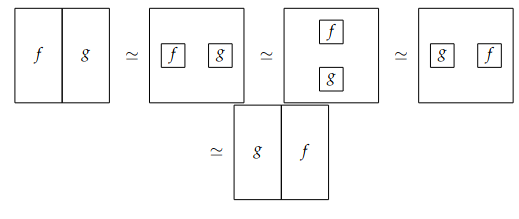
\includegraphics[scale = 0.5]{abelian.png}\caption{$f + g \simeq g +f $.}\label{fig:marginfig}\end{figure}
	That is, so long as $n \ge 2$, we can shrink the domain of $f$ and $g$ to smaller cubes (mapping the remaining region to the base point), slide $f$ and $g$ past each other, and then increase the domains back again. 
\end{Rem}
\begin{exercise}{}{}
	Let $G$ be a topological group with identity element $e$, then $\pi_1(G,e)$ is abelian. \\
	\textbf{Hint: } Use Eckmann--Hilton, or note the following: A topological group is a group object in the category of topological spaces. What is a group object in the category of groups? 
\end{exercise}
\begin{Prop}
	If $n \ge 1$ and $X$ is path connected then there is an isomorphism $\beta_{\gamma} : \pi_n(X, x_0) \xrightarrow{\simeq} \pi_n(X, x_0)$ given by $\beta_{\gamma}([ f ]) = [\gamma \circ f ]$ where $\gamma$ is a path in $X$ from $x_1$ to $x_0$ and $\gamma \circ f$ is constructed by first shrinking the domain of $f$ to a smaller cube inside of $I^n$, and then inserting the path $\gamma$ radially from $x_1$ to $x_0$ on the boundaries of these cubes.
	\begin{figure}[h] \centering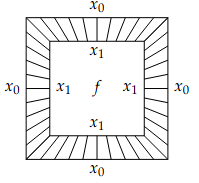
\includegraphics[scale = 0.5]{path.png}\caption{$\beta_{\gamma}$.}\label{fig:marginfig}\end{figure}
\end{Prop}
\begin{proof}
	Observe the following:
	\begin{enumerate}
		\item $\gamma \circ (f + g) \simeq \gamma \circ f + \gamma \circ g$, i.e., $\beta_{\gamma}$ is a group homomorphism.
		\item $(\gamma \circ \eta) \circ f \simeq \gamma \circ (\eta \circ f)$, for $\eta$ a path from $x_0$ to $x_1$. 
		\item $c_{x_0} \circ f \simeq f$, where $c_{x_0}$ denotes the constant path based at $x_0$. 
		\item $\beta_{\gamma}$ is well-defined with respect to homotopies of $f$ or $\gamma$. 
	\end{enumerate}

	The only point that is perhaps not clear is (i). For this, we deform $f$ and $g$ to be constant on the right and left halves of $I^n$, respectively, producing maps we call $f+0$ and $0 + g$. We then excise a wider symmetric middle slab of $\gamma(f+0)$  and $\gamma(0+g)$ until it becomes $\gamma(f+g)$:
\begin{figure}[h] \centering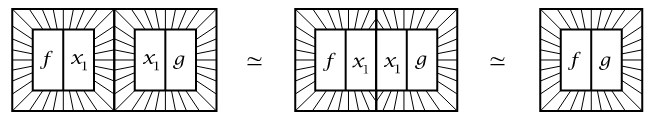
\includegraphics[scale = 0.5]{path_invariance.png}\end{figure}
\end{proof}
\begin{Rem}
	Therefore if $X$ is path-connected, different choices of base point $x_0$ yield isomorphic groups $\pi_n(X,x_0)$, which may then simply be written as $\pi_n(X)$. 
\end{Rem}
\begin{Lem}
	If $\{ X_{\alpha} \}$ is a collection of path-connected spaces, then $\pi_n(\prod_{\alpha} X_{\alpha}) \cong \prod_{\alpha} \pi_n(X_{\alpha})$. 
\end{Lem}
\begin{proof}
	Note that $\Hom(Y,\prod_{\alpha} X_{\alpha}) \simeq \prod_{\alpha} \Hom(Y,X_{\alpha})$. In particular, a map $S^n \to \Hom(Y,\prod_{\alpha}X_{\alpha})$ is determined by a collection of maps $S^n \to X_{\alpha}$. Likewise, a homotopy $S^n \times I \to \prod_{\alpha} X_{\alpha}$ is determined by a colletion of homotopies $S^n \times I \to X_{\alpha}$. This implies the result. 
\end{proof}
\begin{Prop}
	Homotopy groups are functorial: given a map $\phi \colon X \to Y$ we get group homomorphisms $\phi_{\ast} \colon \pi_n(X,x_0) \to \pi_n(X,\phi(x_0))$ given by $[f] \mapsto [\phi \circ f]$ for all $n \ge 1$. 
\end{Prop}
\begin{proof}
We have the following:
	\begin{enumerate}
	\item $\phi_*$ is well-defined: if $f \simeq g$ via $\psi_t$, then $\phi \circ \psi_t$ defines a homotopy between $\phi \circ f$ and $\phi \circ g$. 
	\item This is a group homomorphism: $\phi \circ (f+g) \simeq \phi \circ g + \phi \circ g$ by the definition of the addition operation. Therefore. 
	\[
\phi_*[f+g] = \phi_*[f] + \phi_*[g]. 
	\]
\end{enumerate}
\begin{exercise}{}{}
	If $\phi \colon X \to Y$ is homotopy equivalence (not necessarily base-point preserving), then $\pi_* \colon \pi_n(X,x_0) \to \pi_n(Y,\phi(y_0))$ is an isomorphism.  
\end{exercise}
\end{proof}
\begin{Rem}
	We recall the following lifting property: Suppose $p \colon (\tilde X,\tilde x_0) \to (X,x_0)$ is a covering, and there is a map $f \colon (Y,y_0) \to (X,x_0)$ with $Y$ path-connected and locally path-connected. Then a lift $\tilde f$ exists if and only if $f_*\pi_1(Y,y_0) \subseteq p_*\pi_1(\tilde X,\tilde x_0)$. 
	% https://q.uiver.app/?q=WzAsMyxbMCwxLCIoWSxZXzApIl0sWzEsMSwiKFgseF8wKSJdLFsxLDAsIihcXHRpbGRlIFgseF8wKSJdLFswLDEsImYiXSxbMiwxXSxbMCwyLCJcXHRpbGRlIGYiLDAseyJzdHlsZSI6eyJib2R5Ijp7Im5hbWUiOiJkYXNoZWQifX19XV0=
\[\begin{tikzcd}
	& {(\tilde X,\tilde x_0)} \\
	{(Y,y_0)} & {(X,x_0)}
	\arrow["f", from=2-1, to=2-2]
	\arrow["p",from=1-2, to=2-2]
	\arrow["{\tilde f}", dashed, from=2-1, to=1-2]
\end{tikzcd}\]

\end{Rem}
\begin{Prop}
	If $p$ is a covering, then $p_* \colon \pi_n(\tilde X,\tilde x_0) \to \pi_n(X,x_0)$ is an isomorphism for all $ n \ge 2$. 
\end{Prop}
\begin{proof}
Let us first show surjectivity. To that end, suppose we have a map $f \colon (S^n,s_0) \to (X,x_0)$ where $n \ge 2$. The assumption on  $n$ gives $\pi_1(S^n) = 0$, so $f_*\pi_1(S^n,s_0) \subseteq \pi_*\pi_1(\tilde X,\tilde x_0)$ holds. We therefore find a lift in the following:
\[\begin{tikzcd}
	& {(\tilde X,\tilde x_0)} \\
	{(S^n,s_0)} & {(X,x_0)}
	\arrow["f", from=2-1, to=2-2]
	\arrow["p", from=1-2, to=2-2]
	\arrow["{\tilde f}", dashed, from=2-1, to=1-2]
\end{tikzcd}\]
Then $p_*[\tilde f] = [f]$, and $p_*$ is surjective. 

To see that $p_*$ is injective, let $[\tilde f] \in \ker(p_*)$, i.e., $p_*[\tilde f] = [p \circ \tilde f] = 0$. Let $f = p \circ \tilde f$, then this is homotopic to the constant map $f \simeq c_{x_0}$ via a homotopy $\phi_t \colon (S^n,s_0) \to (X,x_0)$with $\phi_1 =f $ and $\phi_0 = c_{x_0}$. By the same argument as above, the homotopy $\phi_t$ can be lifted to $\tilde \phi_t$. This satisfies $p \circ \tilde \phi_1 \simeq \phi_1 $ and $p \circ \tilde \phi_0 \simeq \phi_0$. By the uniqueness of lifts, we must have $\tilde \phi_1 \simeq \tilde f$ and $\tilde \phi_0 \simeq c_{x_0}$. In other words, $\tilde \phi_t$ gives a homotopy between $\tilde f$ and $c_{x_0}$, so that $[\tilde f]  = 0$, and $p_*$ is injective. 
\end{proof}
\begin{Exa}
	$S^1$ has universal cover $p \colon \mathbb{R} \to S^1$, $p(t) = e^{2\pi i t}$. Then $\pi_n(S^1) \cong \pi_n(\mathbb{R}) \cong 0$ for $n \ge 2$. 
\end{Exa}
\begin{exercise}{}{}
	Find two spaces $X,Y$ with $\pi_nX \cong \pi_nY$ but $X \not \simeq Y$. 

	\textbf{Hint: } What is the universal cover of $\mathbb{R}P^n$?
\end{exercise}
\begin{Rem}[Relative homotopy groups]
	Suppose we have $(X,x_0)$ and a subspace $A$ containing $x_0$. We note that $i_* \colon \pi_n(A,x_0) \to \pi_n(X,x_0)$ is not injective in general (example, take $S^1$ into $\mathbb{R}^2$). An element in the kernel of $i_*$ is a map $f \colon (I^n,\partial I^n) \to (A,x_0)$ such that 
	\[
(I^n,\partial I^n) \xrightarrow{f} (A,x_0) \xrightarrow{i} (X,x_0)
	\] 
	is homotopic to $c_{x_0}$. This means there exists a homotopy
	\[
H \colon I^n \times I \to X
	\]
	such that $H(-,1) = f, H(-,0) = c_{x_0}$ and $H \mid_{\partial I^n \times I} = c_{x_0}$. 

	If we define $J^n = I^n \times \{ 0 \} \cup \partial I^n \times I \subseteq I^n \times I$, then this is a map of triples
	\[
H \colon (I^{n+1},\partial I^{n+1},J^n) \to (X,A,x_0). 
	\] 
\end{Rem}
\begin{Def}
	\[
\pi_n(X,A,x_0) = [(I^n,\partial I^n,J^{n-1}),(X,A,x_0)]
	\]
\end{Def}
\begin{Rem}
	Equivalently, 
	\[
\pi_n(X,A,x_0) = [(D^n,S^{n-1},s_0),(X,A,x_0)]
	\]
\end{Rem}
\begin{Prop}
	If $n \ge 2$, then $\pi_n(X,A,x_0)$ is a group, and if $n \ge 3$, then it is abelian. 

	For all $n \ge 2$, a map of pairs $\phi \colon (X,A,x_0) \to (Y,B,y_0)$ induces homomorphisms $\phi_* \colon \pi_n(X,A,x_0) \to \pi_n(Y,B,y_0)$ for all $n \ge 2$. 
\end{Prop}
\begin{Thm}\label{thm:les_rel}
	The relative homotopy groups $(X,A,x_0)$ fit into a long exact sequence 
	\[
\cdots \to \pi_n(A,x_0) \xr{i_*} \pi_n(X,x_0) \xr{j_*} \pi_n(X,A,x_0) \xr{\partial_n} \pi_{n-1}(A,x_0) \to \cdots
	\]
	where the map $\partial_n$ is defined by $\partial_n([f]) = [f\mid_{I^{n-1}}]$. 
\end{Thm}
The proof relies on the following.
\begin{Lem}[Compression criterion]
	A map $f \colon (D^n,S^{n-1},x_0) \to (X,A,x_0)$ represents 0 in $\pi_n(X,A,x_0)$ if and only if $f \sim g \text{ rel } S^{n-1}$, where $g$ is a map whose image is contained entirely in $A$. 
\end{Lem}
\begin{proof}
	Suppose $[f] = [g]$ with $g$ as in the statement of the lemma. Note that there is a deformation of $D^n$ onto $x_0$, and so $[f] = [g] = 0$ in $\pi_n(X,A,x_0)$. 

	Conversely, suppose that $[f]$ represents 0 in $\pi_n(X,A,x_0)$. This means there exists a homotopy, relative to $S^{n-1}$, $F \colon D^n \times I \to X$ with $F \mid_{D^n \times \{0 \}} = f$, $F \mid_{D^n \times 1} = c_{x_0}$ and $F \mid_{S^{n-1} \times I} \subseteq A$. We can restrict $F$ to a family of $n$-disks in $D^n \times I$ starting with $D^n \times \{ 0 \}$ and ending with the disk $D^n \times \{1 \} \cup S^{n-1} \times \{ 1\}$, all the disks in the family having the same boundary, then we get a homotopy from $f$ to a map in $A$, stationary on $S^{n-1}$ (said in other words, we can deformation retract $D^n \times [0,1]$ onto $D^n \times \{1 \} \cup S^{n-1} \times I$). 
\end{proof}
\begin{proof}[Proof of \Cref{thm:les_rel}]
	\textbf{Step 1. }Let us first show exactness at $\pi_n(X,x_0)$. \\

	We first show $\im(i_*) \subseteq \ker(j_*)$. Note that $j_*i_*$ is induced by the composition $j \circ i$ and that these are both inclusion maps. Therefore, for $[f] \in \pi_n(A,x_0)$ we have $j_*i_*[f] = [j \circ i \circ f]$, but this has image contained in $A$, and so $j_*i_*[f] = 0$. This shows $\im(i_*) \subseteq \ker(j_*)$. 

	To see the converse (namely, $\ker(j_*) \subseteq \im(i_*)$) let $[f] \in \ker(j_*)$, i.e. $[j \circ f] = 0$. Note that again $j$ is an inclusion map, and by the compression criteria $f \simeq g'$ relative to $S^{n-1}$, where $g'$ has image contained in $A$. Since $x_0 \in S^{n-1}$, the homotopy fixes the basepoint, i.e, $[f] = [g'] \in \pi_n(X,x_0)$. But because $g'$ has image in $A$, $[g'] \in \pi_n(A,x_0)$ and $i_*[g'] = [i \circ g'] = [f]$, so $[f] \in \im(i_*)$. 

	\textbf{Step 2. } Let us now show exactness at $\pi_n(X,A,x_0)$. \\

	Note that the composite $\partial \circ j_* = 0$ since the restriction of a map $(I^n,\partial I^n,J^{n-1}) \to (X,x_0,x_0)$ to $I^{n-1}$ has image $x_0$ and so represents $0$ in $\pi_{n-1}(A,x_0)$. Therefore, $\im(j_*) \subseteq \ker(\partial)$. For the converse, suppose $[f] \in \ker(\partial)$. This means there exists a basepoint preserving homotopy $H \colon I^{n-1} \times I \to A$ (relative to $\partial I^{n-1}$) from $f \mid_{I^{n-1} \times \{ 0 \}}$ to the constant map where the image of $H$ is contained entirely in $A$. We can then define another homotopy $H$, such that $G_0 = f$, $G_t \mid_{I^{n-1}} = H_t$ and the rest of the image of $G_t$ is $f[I^n]$ union with the image of $H_s$ for $0 \le s \le t$. This homotopy maps $S^{n-1}$ into $A$ at all times, so $[f] = [G_1]$. Morevoer, $G_1$ maps the boundary of $I^n$ to $x_0$, so $[G_1] \in \pi_n(X,x_0)$. Altogether, 
	\[
j_*[G_1] = [j \circ G_1] = [G_1] = [f]
	\]
	so $\ker(\partial) \subseteq \im(j_*)$. 


\textbf{Step 3:} Exactness at $\pi_n(A,x_0)$.
	
	Let $[f] \in \pi_n(X,A,x_0)$ then $i_*\partial \in \pi_{n-1}(X,x_0)$ is the class represented by $f \mid_{I^{n-1}}$ and this is homotopic relative $J^{n-2}$ to the consant map to $x_0$, via $f$ viewed as a homotopy. So this implies $\im(\partial_*) \subseteq \ker(i_*)$. Conversely, let $[f] \in \ker(i_*)$ i.e., $i_*[f]= [i \circ f]= 0$. Therefore, there exists a homotopy $H$ between $f$ and a constant map through a homotopy that has image in $X$ and preserves $x_0$. Since $H_0 = f$ has image in $A$ and $H_1$ has image $\{x_0\}$, and $H_0$ takes the boundary to $\{ x_0 \}$, we see that $[H] \in \pi_n(X,A,x_0)$, and moreover $\partial([H]) \simeq f$. Therefore, $[f] \in \im(\partial)$, and $\im(\partial) = \ker(i_*)$. 
\end{proof}
\begin{Def}
	A pair $(X,A)$ with basepoint $x_0$ is said to be $n$-connected if $\pi_i(X,A) = 0$ for all $i \le n$. 
\end{Def}
\begin{Lem}
	A pair $(X,A)$ is $n$-connected if and only if $\pi_i(A) \xr{i_*} \pi_i(X)$ is an isomorphism for $i < n$ and a surjection for $i = n$. 
\end{Lem}
\begin{proof}
	Use the long exact sequence in homotopy. 
\end{proof}
\begin{exercise}{}{}
Let $X$ be a path-connected space, and $CX$ the cone on $X$. Show that 
	\[
\pi_n(CX,X,X_0) \cong \pi_{n-1}(X,x_0)
	\]
	for $n \ge 1$. 
\end{exercise}

\end{document}